%!TEX root = pdl.tex

\section{Processus de gestion}
\subsection{Délais}
La livraison du produit fini est prévue pour le mecredi 6 Mai.

\subsection{Détail des différentes taches}
\subsubsection{Diagramme PERT et GANTT}
\begin{figure}[thbp]
	\centering
		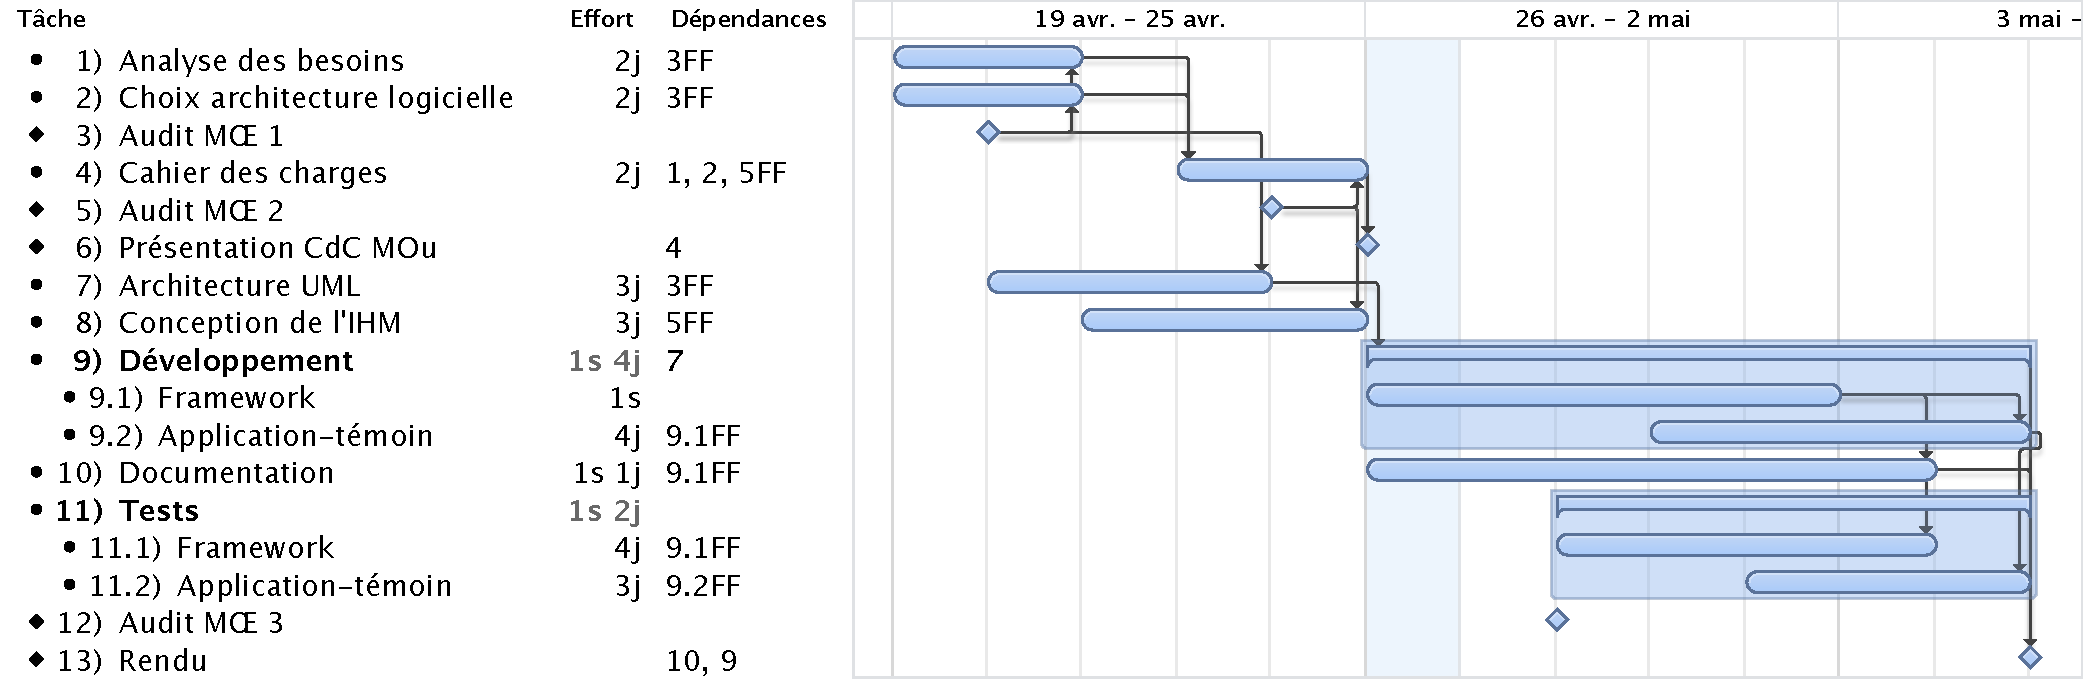
\includegraphics[height=7cm,angle=90]{../diagrammes/planification.pdf}
	\caption{Diagramme PERT}
	\label{fig:pert}
\end{figure}
La figure~\ref{fig:pert}, p.~\pageref{fig:pert} donne le détail de la réalisation des différentes tâches, leurs dépendances et leur ordonnancement. En complément, le diagramme de Gantt décrit leur planification.

\subsection{Processus de contrôle et de suivi}

Le suivi et le contrôle du projet sera quotidiennement effectué au travers de réunions dans lesquelles seront relevés : 
\begin{itemize}
 \item l'avancement général du projet
 \item l'affectation des nouvelles taches
\end{itemize}

Ces audits avec le maître d’oeuvre Mr François Puitg permettront d'effectuer des mesures précises du temps consacré au projet.


%\subsection{Plan de projet}
%\subsubsection{Planification des phases}
%\subsubsection{Objectifs d’itération}
%\subsubsection{Version}
%\subsubsection{Calendrier du projet}
%\subsubsection{Ressources humaines du projet}

%\subsection{Suivi de projet et contrôle}
%\subsubsection{Gestion des exigences}
%\subsubsection{Contrôle de la qualité}
%\subsubsection{Rapports et mesures}
%\subsubsection{Gestion de risque}
%\subsubsection{Gestion de configuration}
